
%%%%%%%%%%%%%%%%% Introduction to the Assignment %%%

In this Assignment, \textit{\textbf{Problem 3 - Propagation Effects \& Targets}}, ...


%%%%%%%%%%%%%%%%% TASK 1 %%%
\section{Radar Performance}

\subsection{Phenomena affecting radar performance}
The performance of a radar is affected by couple of different phenomena, which degrade or attenuate the sent and received signal.
\begin{enumerate}
	\item Atmospheric attenuation
			Atmospheric attenuation is a major loss term, since the radar beam is attenuated as it's travelling through the atmosphere and its constituents (2-way-loss).
			Water vapor, e.g. clouds, rain or fog, and its density as well as temperature are playing a major role in attenuating the signal. This attenuation is also frequency dependant, e.g. higher frequencies are more attenuated, c.f. fig \ref{fig:attenuation}.
			\begin{figure}[!htbp]
			\centering
			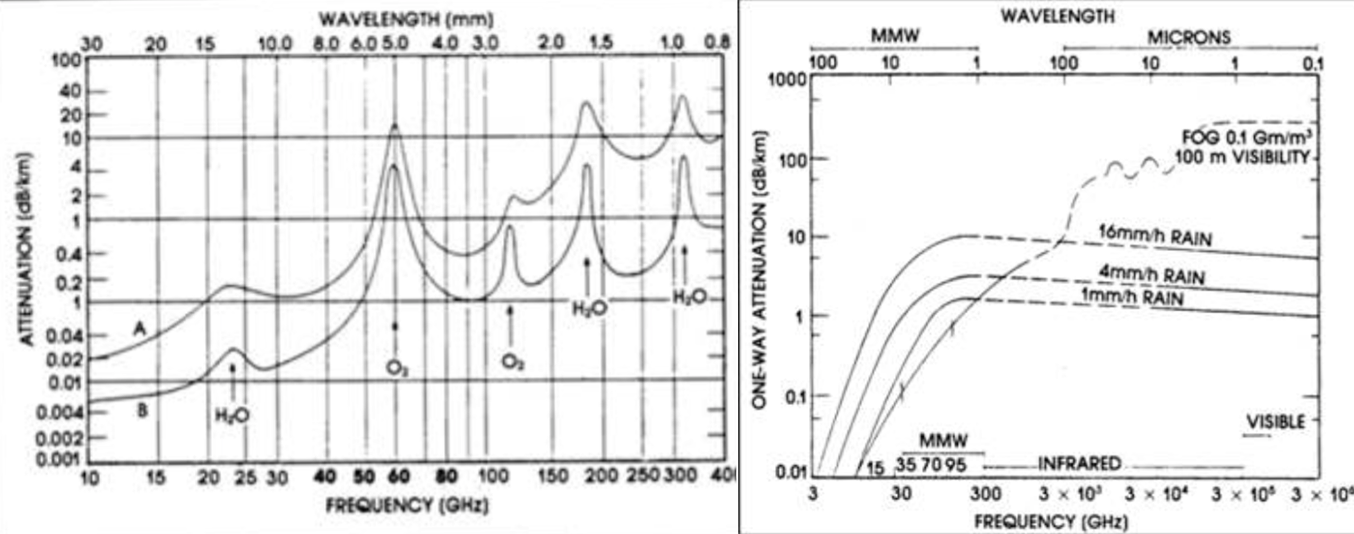
\includegraphics[width=0.9\textwidth]{images/attenuation}
			\caption{atmospheric attenuation as function of frequency \citep{erickson:lecture}}
			\label{fig:attenuation}
			\end{figure}
	\item Surface reflection
			Surface reflection, the reflection of an EM-wave off earth's surface, can lead to multi-path effects when the receiver is hit by the reflected EM-wave, thus leading to measurements that do not correspond with the direction of the original radar beam (assuming an atmospheric radar).
	\item Diffraction
			Diffraction describes the process, when an EM-wave hits an obstacle and is bend around its corners, thus the EM-wave can illuminate things even in a so-called \textit{"shadow zone"}, the zone behind an obstacle. In radar terms, this particular effect can be used to extend the range even beyond the horizon for lower frequencies, since for higher frequencies the diffraction is not very effective.
	\item Refraction
			Atmospheric Refraction is the "bending" of an EM-wave as it propagates through the atmosphere. Refraction is dependant on the constituent of the penetrated material, but also on the thickness of the material and the wavelength of the beam, since the refractive index changes with frequency (optical dispersion) \citep{erickson:lecture}.
	
\end{enumerate}



\subsection{22 GHz and 60 GHz Operation}
Radar is seldom used at 22GHz or 60GHz since at these frequencies the atmosphere is vastly attenuating the signal. Components responsible for the absorption in case of 22GHz is Oxygen ($O_2$) and at 60GHz water vapour ($H_2O$), c.f. fig. \ref{fig:absorb}.
\begin{figure}[h!]
	\centering
	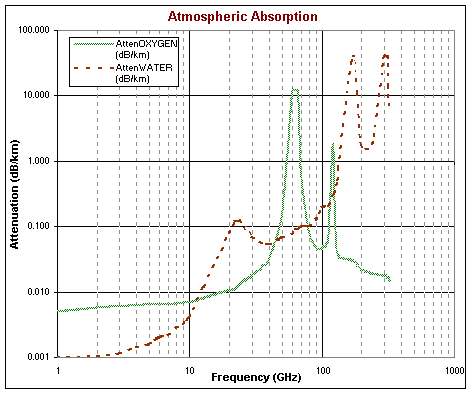
\includegraphics[width=0.7\linewidth]{images/absorbtion}
	\caption{Atmospheric attenuation of different frequencies \protect\footnotemark}	
	\label{fig:absorb}
\end{figure}
\footnotetext{source: \href{http://www.rfcafe.com/references/electrical/images/atm_absorption.gif}{RFCafe}}



%%%%%%%%%%%%%%%%% TASK 2 %%%
\section{Radar cross section (RCS)}

\subsection{Behaviour of normalized RCS}

\subsection{Low specular RCS}


%%%%%%%%%%%%%%%%% TASK 3 %%%
\section{Radar parameters affecting performance}

\subsection{Pulse width}

\subsection{Antenna Gain}

\subsection{Transmitter Power}

\subsection{Number of pulses returned from the target}

\subsection{System losses}

\subsection{Sensitivity of maximum range to RCS changes}

%%%%%%%%%%%%%%%%% TASK 4 %%%
\section{Atmospheric studies with MF \& HF radars}

\subsection{Coherent Echoes at 50-110km}

\subsection{Choice of operational frequency \& optimal PRF}

\subsection{Main Principle of space antenna techniques}

\subsection{Apparent and true velocity}

\subsection{Deficiency of full correlation analysis for MF/HF}

